\section{RTDroid}
RTDroid si pone l'obiettivo di aggiungere supporto real-time ad Android nella sua interezza. Questo significa che tutti i problemi sopra riportati devono essere corretti in modo da fornire un supporto completo e che dia garanzie solide. In questa estensione, solamente un processo di livello utente (l'applicazione) è in esecuzione. 

Per risolvere tutti i problemi di Android è necessario un redesign profondo che arriva fino al livello del kernel. Quest'ultimo viene sostituito con un kernel real-rime, LinuxRT o, meglio, RTEMS. Anche la VM di Android viene sostituita, con Fiji. Sopra questo nuovo strato vengono offerte le ''classiche'' API Android, con l'aggiunta di una serie di estensioni che correggono specifici problemi riscontrati. Queste API aggiuntive rispettano la RTSJ. 

\subsection{Looper e Handler}
Ad ogni messaggio viene assegnata una priorità, attraverso due modalità:
\begin{itemize}
	\item\textit{inheritance}: il messaggio eredita la priorità del mittente;
	\item\textit{inheritance + specified}: il mittente può specificare una priorità relativa a tutti i messaggi inviati.
\end{itemize}
Dopodiché viene definita una coda per ogni priorità, con associata un \texttt{Looper} e un \texttt{Handler}. Messaggi a priorità più bassa non ritarderanno quelli a priorità più alta. Per avere garanzie sulla quantità di memoria utilizzata, le code possono essere dimensionate staticamente.

\subsection{AlarmManager}
Sia la registrazione che la consegna devono essere ridefinite per un completo supporto real-time. Per la registrazione vengono utilizzati degli alberi rosso neri (Figura~\ref{fig:rtalarm}), così da rendere il processo prevedibile sulla base della complessità delle operazioni sull'albero. 
\begin{figure}[h]
	\centering
	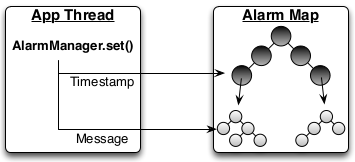
\includegraphics[width=0.7\linewidth]{rtalarm}
	\caption{Registrazione di allarmi real-time}
	\label{fig:rtalarm}
\end{figure}

L'albero principale mantiene i timestamp delle registrazioni e dei puntatori ad altri alberi, che ordinano i timestamp sulla base della priorità del richiedente. Di conseguenza una registrazione include solamente due inserimenti. Organizzando gli alberi in base alla priorità si ha la garanzia che un messaggio diretto ad un thread a bassa priorità non ritardi uno a priorità più alta. In questo modo, anche se un thread a bassa priorità registra un sacco di eventi (più di quanti ne possono essere gestiti), i thread a priorità più alta non verranno in nessun modo toccati.

Per la consegna viene definito un \texttt{AlarmManager} thread a cui è assegnata la priorità più alta di tutte. Questo thread sostituisce il classico meccanismo di invio di messaggi di Android. Si sveglia ogni volta che c'è un inserimento in un albero rosso nero e pianifica un thread all'istante temporale specificato. A quest'ultimo viene associata la callback specificata dall'applicazione.

\subsection{SensorManager}
Il sensing funziona attraverso un \textit{polling thread} che periodicamente ascolta l'ambiente circostante. Questo comunica con vari \textit{processing thread}, uno per ogni sensore, che interpretano i dati ricevuti dal polling thread.

I problemi riportati vengono risolti attraverso \textit{priority inheritance}. Quando un thread con priorità \texttt{p} registra un listener per un sensore, al thread associato a quel sensore viene assegnata la priorità \texttt{p}. Se più di un thread si associano allo stesso sensore, allora al thread del sensore è associata la priorità più alta tra tutti. Anche i thread creati per eseguire le callback hanno assegnata la priorità \texttt{p}. Il polling thread ha la priorità più alta di tutte, in modo da assicurare che i dati vengano raccolti appena possibile.

Quando un'applicazione registra un nuovo listener per un sensore viene di fatto creato un nuovo percorso di consegna dal polling thread al listener. Questo percorso è isolato ed eredita la priorità del thread che l'ha creato. 

\subsection{Sostituire componenti non real-time con componenti real-time}
Il kernel Linux di Android ha molte modifiche per renderlo adatto all'utilizzo in un ambiente con risorse limitate. Questo diventa un problema quando si cerca di sostituire alcuni componenti per migliorare il supporto real-time.

\paragraph{Bionic.} Un esempio è dato dalle librerie C native. Al posto di \texttt{glibc} Android utilizza \textit{Bionic}. Bionic è una libreria C leggera e altamente semplificata ed ottimizzata in modo da poter essere utilizzata in ambienti con risolrse limitate, in particolare CPU a bassa frequenza e poca memoria. Sfortunatamente però non aderisce alla specifica POSIX e non supporta le estensioni real-time di mutex e pthreads. Una modifica di questa libreria è necessaria per utilizzare una VM real-time, come Fiji.

\paragraph{Patch del kernel incompatibili.} Android ha introdotto molte modifiche al kernel Linux, tanto che l'applicazione automatica di patch per ottenere RTLinux è impossibile, e deve essere fatta manualmente. Anche dopo averla fatta manualmente, comunque, il kernel rimane non completamente prerilasciabile e questo comporta alti tempi di attesa possibili. 

\paragraph{Funzionalità non real-time del kernel.} Il kernel Android ha due funzionalità critiche sotto l'aspetto real-time. La prima è l'\textit{out of memory killer} (OOM), che viene avviato in condizioni di bassa memoria disponibile. Analizza tutte le pagine di memoria per verificare che il sistema sia veramente in condizioni critiche ed uccide un processo selezionato. I thread in esecuzione vengono fermati e bloccati per un periodo di tempo variabile. In un contesto dove è permessa solo l'esecuzione di un processo utente, però, OOM è inutile.

